% Report for the Solar Filament Segmentation Challenge 2026, in the organisers' template (acmart, sigconf).
% preamble.tex and the first two entries of main.bib come from the template unchanged.
% Build: pdflatex main && bibtex main && pdflatex main && pdflatex main
\documentclass[sigconf]{acmart}
% =============================================================================
% Template setup — participants normally do not edit this file.
% Author content belongs in main.tex; citations belong in main.bib.
% \documentclass lives in main.tex so Overleaf does not treat this file as root.
% =============================================================================

% --- Competition / non-ACM-submission friendly rights metadata -------------
\setcopyright{none}
\settopmatter{printacmref=false}
\acmConference[Kaggle Competition]{Filament Segmentation Challenge}{2026}{\href{https://www.kaggle.com/competitions/filament-segmentation-2026}{kaggle.com/competitions/filament-segmentation-2026}}
\acmBooktitle{Competition Report}
\acmDOI{}
\acmISBN{}

% --- Author guidance text --------------------------------------------------
% \guide{...} is gray italic while \guideStyletrue; omitted from the PDF if false.
% Flip the switch in main.tex after % =============================================================================
% Template setup — participants normally do not edit this file.
% Author content belongs in main.tex; citations belong in main.bib.
% \documentclass lives in main.tex so Overleaf does not treat this file as root.
% =============================================================================

% --- Competition / non-ACM-submission friendly rights metadata -------------
\setcopyright{none}
\settopmatter{printacmref=false}
\acmConference[Kaggle Competition]{Filament Segmentation Challenge}{2026}{\href{https://www.kaggle.com/competitions/filament-segmentation-2026}{kaggle.com/competitions/filament-segmentation-2026}}
\acmBooktitle{Competition Report}
\acmDOI{}
\acmISBN{}

% --- Author guidance text --------------------------------------------------
% \guide{...} is gray italic while \guideStyletrue; omitted from the PDF if false.
% Flip the switch in main.tex after % =============================================================================
% Template setup — participants normally do not edit this file.
% Author content belongs in main.tex; citations belong in main.bib.
% \documentclass lives in main.tex so Overleaf does not treat this file as root.
% =============================================================================

% --- Competition / non-ACM-submission friendly rights metadata -------------
\setcopyright{none}
\settopmatter{printacmref=false}
\acmConference[Kaggle Competition]{Filament Segmentation Challenge}{2026}{\href{https://www.kaggle.com/competitions/filament-segmentation-2026}{kaggle.com/competitions/filament-segmentation-2026}}
\acmBooktitle{Competition Report}
\acmDOI{}
\acmISBN{}

% --- Author guidance text --------------------------------------------------
% \guide{...} is gray italic while \guideStyletrue; omitted from the PDF if false.
% Flip the switch in main.tex after \input{preamble}.
%
% Do not use \guide{...} for \email{...}.
\usepackage{xcolor}
\newif\ifguideStyle
\guideStyletrue
\newcommand{\guide}[1]{%
  \ifguideStyle
    {\color{gray!65}\itshape #1}%
  \fi
}

% --- Math ------------------------------------------------------------------
% Do NOT load amssymb (or amsfonts): acmart already loads newtxmath, which
% defines the same symbols (e.g. \Bbbk) and causes a conflict on Overleaf.
% amsmath is already provided by acmart; mathtools extends it.
\usepackage{mathtools}

% --- Figures ---------------------------------------------------------------
% graphicx is already loaded by acmart
\usepackage{subcaption}

% --- Tables ----------------------------------------------------------------
% booktabs is already loaded by acmart
\usepackage{tabularx}
\usepackage{multirow}

% --- Bibliography style is set in main.tex (ACM-Reference-Format) ----------
.
%
% Do not use \guide{...} for \email{...}.
\usepackage{xcolor}
\newif\ifguideStyle
\guideStyletrue
\newcommand{\guide}[1]{%
  \ifguideStyle
    {\color{gray!65}\itshape #1}%
  \fi
}

% --- Math ------------------------------------------------------------------
% Do NOT load amssymb (or amsfonts): acmart already loads newtxmath, which
% defines the same symbols (e.g. \Bbbk) and causes a conflict on Overleaf.
% amsmath is already provided by acmart; mathtools extends it.
\usepackage{mathtools}

% --- Figures ---------------------------------------------------------------
% graphicx is already loaded by acmart
\usepackage{subcaption}

% --- Tables ----------------------------------------------------------------
% booktabs is already loaded by acmart
\usepackage{tabularx}
\usepackage{multirow}

% --- Bibliography style is set in main.tex (ACM-Reference-Format) ----------
.
%
% Do not use \guide{...} for \email{...}.
\usepackage{xcolor}
\newif\ifguideStyle
\guideStyletrue
\newcommand{\guide}[1]{%
  \ifguideStyle
    {\color{gray!65}\itshape #1}%
  \fi
}

% --- Math ------------------------------------------------------------------
% Do NOT load amssymb (or amsfonts): acmart already loads newtxmath, which
% defines the same symbols (e.g. \Bbbk) and causes a conflict on Overleaf.
% amsmath is already provided by acmart; mathtools extends it.
\usepackage{mathtools}

% --- Figures ---------------------------------------------------------------
% graphicx is already loaded by acmart
\usepackage{subcaption}

% --- Tables ----------------------------------------------------------------
% booktabs is already loaded by acmart
\usepackage{tabularx}
\usepackage{multirow}

% --- Bibliography style is set in main.tex (ACM-Reference-Format) ----------


\guideStylefalse
\graphicspath{{figures/}}
\emergencystretch=1.5em

\begin{document}

\title[One Network and Two Keep-Scorers]{Segmenting Solar Filaments When the Annotators Disagree: One Network and Two Keep-Scorers}
\subtitle{A Solution to the Solar Filament Segmentation Challenge 2026} % DO NOT CHANGE

\author{Muhammad Elias Muhammadi}
\affiliation{%
  \institution{Independent Researcher}
  \country{}
}

\begin{abstract}
    This report describes our solution to the Solar Filament Segmentation Challenge~2026, a Kaggle competition on automatic segmentation of solar filaments in GONG H-$\alpha$ observations.
    I first measured what the labels allow: two annotators of the same frame agree with a
    Panoptic Quality (PQ) of 0.34, and the mean of their masks scores 0.78 against them. The
    pipeline that follows from this is small. One ConvNeXt-T U-Net predicts, at native resolution,
    the probability that an annotator marks a pixel; connected components of the thresholded map
    are the candidates; a boosted-tree scorer and a small CNN on candidate patches estimate the
    IoU each candidate will reach, and a candidate is kept when the estimate exceeds half the
    expected PQ. The out-of-fold PQ on the 707 training frames is 0.459 (90\% interval 0.451 to
    0.467) at 0.35\,s per frame. I did not use the test annotations that are public in the MAGFiLO
    release, and I report the ideas that did not help. Code, weights and a notebook that reproduces
    the submission are at \url{https://github.com/Muhammad-Elias-Muhammadi/Solar-Filament-Segmentation}.
\end{abstract}

\maketitle

% ==================================== %
%              INTRODUCTION            %
% ==================================== %
\section{Introduction}
    This report goes over the details of our submitted solution to the Solar Filament Segmentation Challenge~2026 \cite{filament-segmentation-2026}. The challenge, launched on July~10,~2026, is organized by the Earth-Space AI Research (ESAIR) Lab\footnote{\href{https://www.esairlab.com/home}{www.esairlab.com/}}. This challenge utilizes the MAGFiLO dataset for evaluation of the segmentation algorithms \cite{ahmadzadeh2024dataset}.
The training set has 707 full-disk frames from the six GONG sites~\cite{harvey2011} with 1,154
annotator records and 8,199 filament polygons; 411 frames were drawn by one annotator, 145 by two
and 151 by three. A submission is one set of disjoint masks per frame, scored against each record
of the frame with PQ~\cite{kirillov2019} at IoU $>0.5$, the counts pooled.

Before building anything larger I scored the labels against themselves with the same metric
(Table~\ref{tab:ceiling}). Three things follow. First, the annotators disagree far more than the
models differ: one annotator against another reaches 0.34, and so does the union or intersection
of two against the third. The disagreement is about which faint filaments exist and where a
filament ends (Figure~\ref{fig:qual}b). Second, a submission cannot satisfy two or three
annotators at once, so even the mean of the annotators' own masks stops at 0.78. Third, grouping
pixels into instances is not the difficulty: the connected components of an annotator's own mask
reproduce that annotator's filaments almost exactly, because only 30 of the 8,199 filaments are
drawn in several pieces and 10 touch a neighbour. I therefore dropped the instance detector of my
earlier versions and treated the problem as two questions: what is the probability that an
annotator marks a pixel, and which components of that map are worth keeping.

\paragraph{Related work.} Deep networks have replaced thresholding and region growing for
filament segmentation in H$\alpha$ images: U-Nets and their variants~\cite{zhu2019,liu2021},
detectors that also classify filaments~\cite{guo2022}, and a semi-supervised U-Net that transfers
across observatories~\cite{diercke2024}. A Mask R-CNN on full-disk frames was an early
instance-level approach on GONG data~\cite{ahmadzadeh2019}. These works train against one mask per
image and mostly report pixel scores. Here a frame can carry up to three masks that disagree, and
the score is instance-level and pooled over the annotators. I therefore treat the annotators as a
population to be modelled, in the spirit of learning from individual labelers~\cite{guan2018}, and
choose the output that maximises the expected metric.

\paragraph{Contributions.} (1) A measurement of what the labels allow under the competition
metric (Table~\ref{tab:ceiling}). (2) A keep rule derived from the metric itself: a candidate is
kept exactly when its expected matched IoU exceeds half the PQ. (3) A patch-based CNN scorer which,
averaged with a feature scorer, is the only change to the decoder that helped. (4) Ten ideas that
did not help, each tested through the complete decoder (Table~\ref{tab:neg}).

\begin{table}[t]
\caption{The labels scored against themselves and against my models (PQ, training frames).}
\label{tab:ceiling}
\small
\begin{tabular}{@{}lr@{}}
\toprule
scored against the annotators & PQ \\
\midrule
another annotator of the same frame & 0.340 \\
union / intersection of two, against the third & 0.334 / 0.318 \\
this work, out-of-fold & 0.459 \\
this work with perfect keep decisions & 0.519 \\
mean of the annotators' masks, all frames & 0.745--0.782 \\
\quad frames with one annotator & 1.00 \\
\quad frames with two / three annotators & 0.55--0.71 / 0.56--0.61 \\
components of an annotator's own mask & 0.997 \\
\bottomrule
\end{tabular}
\end{table}

% ==================================== %
%              METHODOLOGY             %
% ==================================== %
\section{Methodology}\label{sec:methodology}

\begin{figure*}[t]
\centering
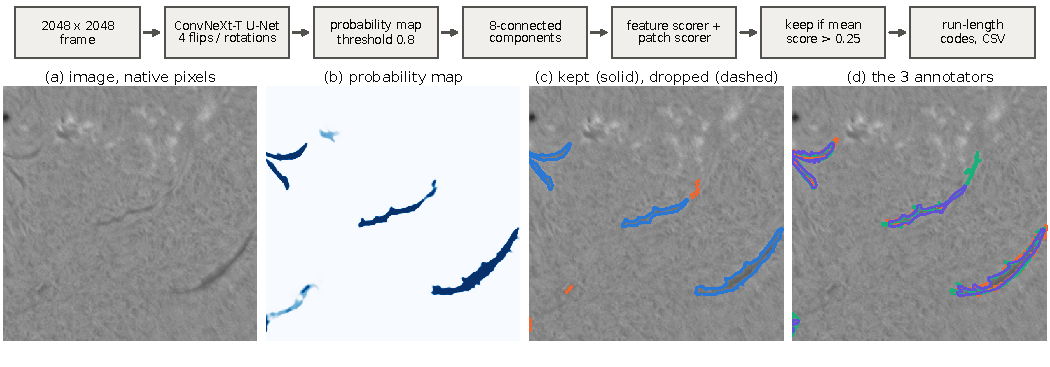
\includegraphics[width=\textwidth]{pipeline.pdf}
\caption{The pipeline (top row) and one $400\times400$ px region of a validation frame going
through it. The network turns the image (a) into a probability map (b). Components above 0.8 are
candidates; the two scorers keep the filaments and drop the small pieces (c). The three
annotators of this frame (d, one colour each) agree on the cores and differ at the ends.}
\label{fig:pipeline}
\end{figure*}

Figure~\ref{fig:pipeline} shows the whole pipeline. It uses existing parts: a
U-Net~\cite{unet,smp} with a ConvNeXt-T encoder~\cite{convnext,timm}, connected components, a
gradient-boosted regressor~\cite{sklearn} and a ResNet-18~\cite{resnet}. What is specific to this
task is the target, the keep rule and the second scorer.

\paragraph{Data, target and splits.} I use only the Kaggle bundle. There is no pre-processing
beyond reading the 8-bit frame; nothing is downsampled, because a filament is often three to six
pixels wide and at half resolution the IoU of such a ribbon is decided by rounding. The target of
a frame is the mean of its annotators' masks, rasterised at $2048\times2048$, so a pixel marked by
one of three annotators has the value $1/3$. I use five folds for training and validation; the
test set is the one of the competition. The folds are built over frames, never over records;
whole 27-day blocks go to one fold because a filament lives for days, and the folds are
stratified by site.

\paragraph{Network and training.} The U-Net has 31.9\,M parameters, one grey input channel and
two outputs: the filament probability and an auxiliary centre line. Each step draws twelve
$1024\times1024$ crops at native scale. The augmentation follows what varies between GONG
frames: zoom by 0.85--1.25, any rotation and flip, gamma, contrast and brightness, Gaussian blur
and a down-and-up resampling for seeing, a smooth multiplicative field for thin cloud, and a
change of the limb darkening. Half of the crops receive one to four real filaments pasted from
other training frames~\cite{copypaste}. The loss is binary cross-entropy on the soft target,
plus 0.5 soft Dice, plus 0.2 of a centre-line term (cross-entropy on the auxiliary head and
skeleton recall~\cite{skeleton} on the main one) that penalises a broken filament. I train with
AdamW, learning rate $3\cdot10^{-4}$ (half of that in the encoder), 5\% warm-up and a cosine
decay, for 150 epochs of 80 steps, and evaluate an exponential moving average of the weights
(decay 0.999). One fold takes about 1.9 hours on an RTX PRO 6000. The submitted model is trained
on all 707 frames with the same recipe.

\paragraph{Candidates.} At test time the whole frame goes through the network in four flipped
and rotated views, the map is set to zero outside the solar disk and thresholded at 0.8, and
every 8-connected component of at least 30 pixels is a candidate. The masks are disjoint by
construction, which the leaderboard requires.

\paragraph{Keep rule.} Adding a candidate to a frame with $n$ records adds its matched IoU to the
numerator of PQ for every record it matches and exactly $n/2$ to the denominator. Keeping it
therefore raises PQ exactly when $y=\frac1n\sum_{r}\mathrm{IoU}_r\,[\mathrm{IoU}_r>0.5]$ is
larger than $\mathrm{PQ}/2$. I estimate $y$ with two regressors and keep a candidate when the mean
of the two estimates exceeds $\tau=0.25$.

The \emph{feature scorer} is the gradient-boosted regressor, on twenty numbers per candidate:
area and shape, statistics of the probability inside it, its darkness against a surrounding ring,
its distance from disk centre and the number of candidates in the frame.

The \emph{patch scorer} is the ResNet-18, and it looks at the candidate. Its input is a 128\,px
patch with six channels: image, probability map and candidate mask in a window of 1.5 times the
bounding box, and the same three in a window of four times the box for context. It is trained
with cross-entropy on the soft target $y$, with flips, rotations and a brightness jitter; three
seeds and the eight symmetries are averaged. The patch is scale-normalised and so loses the
absolute size of the candidate, which the feature scorer keeps; this is one reason the mean of
the two is better than either. Both scorers are fitted on candidates cut from out-of-fold maps.
The kept masks are written as run-length codes. Figure~\ref{fig:qual} shows examples.

\begin{figure*}[t]
\centering
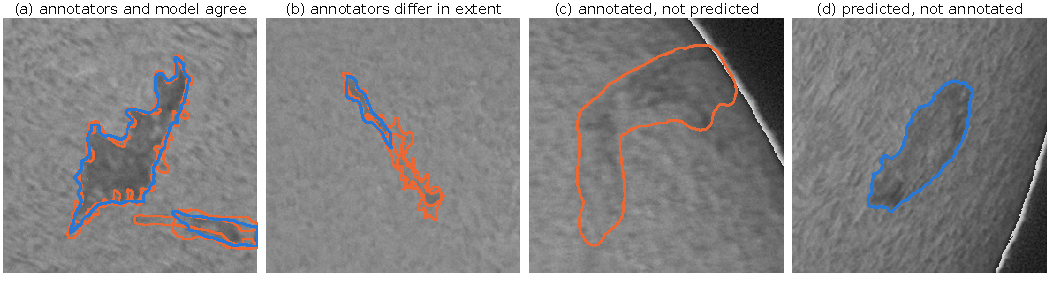
\includegraphics[width=\textwidth]{qualitative.pdf}
\caption{Out-of-fold close-ups, $288\times288$ px. Orange: every annotator of the frame; blue: kept
prediction. (a) A filament with barbs on which the annotators and the model agree. (b) Two
annotators draw the same filament with different extent, and the model follows the shorter outline.
(c) A broad, faint filament at the limb that the only annotator of this frame drew and the model
missed. (d) A dark feature near the limb that the model keeps and no annotator drew; the metric
counts it as a false positive.}
\label{fig:qual}
\end{figure*}

% ==================================== %
%              EVALUATION              %
% ==================================== %
\section{Evaluation}\label{sec:evaluation}

\paragraph{Strategy.} Every number is out-of-fold on the 707 training frames: the network that
drew a mask never saw the frame, and each scorer was fitted on four folds and applied to the
fifth. PQ is pooled over all 1,154 annotator records with my implementation of the metric, which I
tested against the host's self-evaluation notebook. Intervals are 90\% bootstrap intervals over
frames (2,000 resamples). The threshold 0.8 and $\tau$ are the only two numbers tuned on the
pooled out-of-fold score, so the estimate is slightly optimistic. Nothing was tuned on the
leaderboard.

\begin{table}[t]
\caption{Out-of-fold PQ on all 707 frames, built up step by step.}
\label{tab:main}
\small
\begin{tabular}{@{}lr@{}}
\toprule
pipeline & PQ \\
\midrule
previous version: 3 U-Nets, 50 epochs, feature scorer & 0.4455 \\
one ConvNeXt-T U-Net, 150 epochs, components only & 0.402 \\
\quad + feature scorer & 0.4547 \\
\quad + patch scorer instead & 0.4547 \\
\quad + mean of both scorers (submitted) & \textbf{0.4586} \\
\quad\quad 90\% bootstrap interval & 0.451--0.467 \\
\quad\quad lowest and highest fold & 0.447--0.473 \\
\quad with perfect keep decisions (upper bound) & 0.519 \\
\bottomrule
\end{tabular}
\end{table}

\paragraph{Panoptic Quality.} Table~\ref{tab:main} shows the path to the submitted pipeline. The
final result is PQ 0.4586 with segmentation quality 0.683 and recognition quality 0.671 (5,143
matches, 1,981 unmatched predictions, 3,056 unmatched annotations). The model agrees with an
annotator better than a second annotator does (0.34). Teams that published both numbers lose
about 0.06 between out-of-fold and the public board, and my earlier versions did the same, so I
expect about 0.39 to 0.40 there.

\paragraph{IoU, Dice and one-to-many relations.} Figure~\ref{fig:quant} gives the distributions
behind the score. The matched filaments have a mean IoU of 0.683 (median 0.691) and a mean Dice of
0.809 (median 0.818). 855 annotated filaments (10\%) are near misses with a best IoU between 0.3 and
0.5, and 1,849 (23\%) have no predicted mask on them at all: these are mostly faint filaments that
one annotator drew, and keeping more candidates to reach them costs more in false positives than
it returns. Fragmentation and merging are rare. Only 187 annotated filaments (2.3\%) are
covered by two or more predicted masks, and 201 predicted masks (2.8\%) lie over two or more
filaments of the same annotator; 783 predicted masks (11\%) overlap no annotation of the record
they are scored against.

\begin{figure*}[t]
\centering
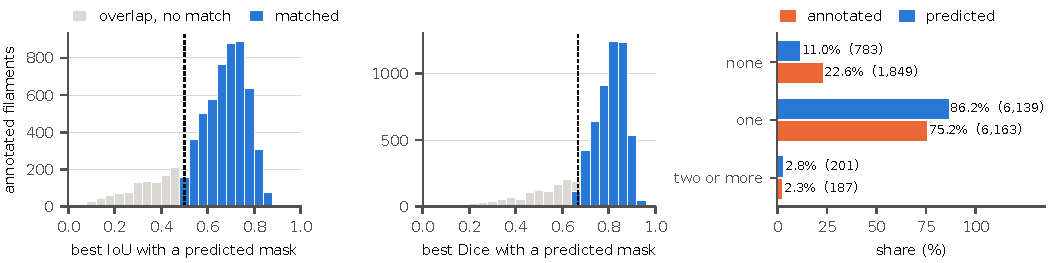
\includegraphics[width=\textwidth]{quantitative.pdf}
\caption{Out-of-fold predictions against all 1,154 annotator records. Left and middle: best IoU and
best Dice of each annotated filament with a predicted mask (the dashed line is the match threshold;
the 1,849 filaments without any overlap are not drawn). Right: how many masks of the other kind
overlap an annotated filament and a predicted mask. ``Two or more'' is fragmentation for the
annotated filaments and merging for the predicted masks.}
\label{fig:quant}
\end{figure*}

\paragraph{What did not help.} Table~\ref{tab:neg} lists what I tested and rejected. Two lessons
were worth more than any single row. The PQ of the raw components is a poor guide: several changes
raised it by up to 0.01 and changed nothing once the scorers had made their decisions, so I
compared every variant through the complete decoder. And averaging a strong map with weaker ones
lowers the score, which is why the submission has one network where my previous version had
three. Longer training was the only change on the network side that survived (+0.009), and the
patch scorer the only one in the decoder (+0.004 here, +0.007 on the maps of the previous
version).

\begin{table}[t]
\caption{Variants I rejected. PQ through the complete decoder; fold~0 (141 frames) unless marked
$^\ast$ (all folds). ``Without'' is the submitted 150-epoch network; the tree row uses the maps of
my previous version and the annotator row the 411 frames with one annotator. On one fold,
differences below 0.005 are noise.}
\label{tab:neg}
\small
\begin{tabular}{@{}lrr@{}}
\toprule
change & without & with \\
\midrule
Jaccard metric loss added & 0.446 & 0.440 \\
ConvNeXt-S encoder & 0.446 & 0.440 \\
input magnified $2\times$ & 0.446 & 0.437 \\
stochastic depth 0.2 & 0.446 & 0.441 \\
three 150-epoch networks averaged & 0.446 & 0.447 \\
six 50-epoch networks averaged & 0.446 & 0.436 \\
labels copied to GONG frames $\pm$2 min & 0.448 & 0.441 \\
extent chosen from a component tree$^\ast$ & 0.446 & 0.437 \\
annotator known to the scorer$^\ast$ & 0.458 & 0.461 \\
crop refiner after the keep rule$^\ast$ & 0.4586 & 0.4600 \\
\bottomrule
\end{tabular}
\end{table}

Three rows deserve a sentence. For the \emph{neighbour frames} I downloaded 1,818 GONG frames
taken within 2.5 minutes of a training frame at the same site, which the organisers allow for
training, checked their alignment (median shift 0.35\,px) and showed each training frame either
as itself or as one of its neighbours. The model was 0.007 worse. The neighbours add new pictures
of the same filaments but no new opinion about them. The \emph{component tree} offers, for each
filament, its outline at eight thresholds. A perfect choice among them would reach 0.57, but
every learned chooser fell back below the single threshold: which extent an annotator draws cannot
be read from the image. The \emph{crop refiner}, a second network that redraws each kept filament
in its own window, moved the mean IoU of the matches from 0.683 to 0.684.

\paragraph{Strengths.} On the three difficulties named by the organisers: \emph{fine structure},
the frame is never downsampled and the masks follow barbs and narrow necks where the annotators
draw them (Figure~\ref{fig:qual}a); \emph{noise}, the augmentation imitates seeing, thin cloud
and limb darkening, and the scorers remove most of the dark specks that survive the threshold
(Figure~\ref{fig:pipeline}c); \emph{continuity}, the centre-line term keeps thin filaments in one
piece, and 2.3\% of the annotated filaments end up fragmented. The pipeline is also cheap. It runs
one network on the full frame and three ResNet-18 scorers on about ten small patches: the 180
test frames take 63\,s on an RTX PRO 6000, that is 0.35\,s per frame including image decoding and
writing the CSV (my previous three-network version needed 0.57\,s). The weights used at test time
are 64\,MB for the network and 69\,MB for the scorers.

\paragraph{Weaknesses and what could improve them.} The model is weak where the annotators are
least consistent: faint, broad filaments near the limb (Figure~\ref{fig:qual}c) and small
filaments that a single annotator marked. It also draws features that look like filaments and
were not annotated (Figure~\ref{fig:qual}d), which the metric penalises. The gap between 0.459
and the 0.519 of perfect keep decisions is what a better scorer could still win, and each of my
attempts at it brought thousandths. I see two ways forward, neither inside this competition's
data: more frames drawn by three annotators, so that the target is a consensus and not one
person's choice, and a scorer that sees the same region a few hours later, since a real
filament persists and a dark speck does not.

\paragraph{Data and rules.} I trained only on the images and polygons of the Kaggle training set,
with encoders pretrained on ImageNet. The 1,818 unlabelled GONG frames were used in one rejected
experiment and are not part of the submission; none of them is a test frame or lies within an
hour of one. I did not download the full MAGFiLO release, which contains annotations of the test
frames, and I used no other ground truth. At test time the pipeline sees only the supplied frame.

\paragraph{Code availability.} The code, the weights of all six networks and of both scorers, the
frozen folds and a notebook that reproduces the submission from the test images are at
\url{https://github.com/Muhammad-Elias-Muhammadi/Solar-Filament-Segmentation}. Running
\texttt{scripts/predict.py} there writes the submitted file byte for byte.

% ==================================== %
%            ACKNOWLEDGMENT            %
% ==================================== %
\section{Acknowledgment}\label{sec:acknowledgment}
    % Do not change
    The organization of the Filament Segmentation Challenge 2026 is partially supported by the U.S. National Science Foundation (NSF) under Grant No. 2209912 and 2433781, directorate for Computer and Information Science and Engineering (CSE), and Office of Advanced Cyberinfrastructure (OAC), and Grant No. 2511630, AST Division Of Astronomical Sciences and MPS Directorate for Mathematical and Physical Sciences.

    The Filament Segmentation Challenge 2026 is sponsored by the U.S. National Science Foundation (NSF) National Solar Observatory (NSO).

    This work utilizes GONG data obtained by the NSO Integrated Synoptic Program, managed by the National Solar Observatory, which is operated by the Association of Universities for Research in Astronomy (AURA), Inc. under a cooperative agreement with the National Science Foundation and with contribution from the National Oceanic and Atmospheric Administration. The GONG network of instruments is hosted by the Big Bear Solar Observatory, High Altitude Observatory, Learmonth Solar Observatory, Udaipur Solar Observatory, Instituto de Astrofísica de Canarias, and Cerro Tololo Interamerican Observatory.

\bibliographystyle{ACM-Reference-Format}
\bibliography{main}

\end{document}
